\documentclass[tikz,border=4pt]{standalone}
\usepackage{amsmath}
\begin{document}
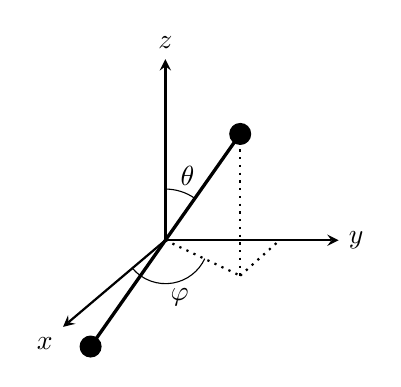
\begin{tikzpicture}[>=stealth, thick, scale=1.0]
  % 3D-like axes
  \draw[->] (0, 0) -- (0, 2.3) node[above] {$z$};
  \draw[->] (0, 0) -- (2.2, 0) node[right] {$y$};
  \draw[->] (0, 0) -- (-1.3, -1.1) node[below left] {$x$};

  % Diatomic molecule endpoints
  \coordinate (A) at (0.95, 1.35);
  \coordinate (B) at (-0.95, -1.35);
  \coordinate (P) at (0.95, -0.45);

  % Projection lines (dotted)
  \draw[dotted, thick] (A) -- (P);
  \draw[dotted, thick] (0, 0) -- (P);
  \draw[dotted, thick] (P) -- (1.45, 0);

  % Molecule bond
  \draw[very thick] (B) -- (A);
  \fill[black] (A) circle (0.14);
  \fill[black] (B) circle (0.14);

  % Angle theta
  \draw[thin] (0, 0.65) arc (90:55:0.65);
  \node at (0.28, 0.82) {$\theta$};

  % Angle phi
  \draw[thin] (-0.42, -0.355) arc (220:335:0.55);
  \node at (0.18, -0.72) {$\varphi$};
\end{tikzpicture}
\end{document}
